\documentclass{report}

% Packages for images.
\usepackage{graphicx}
\usepackage{float}
\usepackage{caption}

% Packages for mathematical formulae/symbols.
\usepackage{amsmath}
\usepackage{amssymb}
\usepackage{amsfonts}

% Packages for code snippets and algorithms.
\usepackage{listings}
\usepackage{xcolor}
\definecolor{codegreen}{RGB}{0,128,0}
\definecolor{codegray}{RGB}{110,110,110}
\definecolor{codepurple}{RGB}{163,21,21}
\definecolor{codeblue}{RGB}{0,0,180}
\definecolor{backwhite}{RGB}{255,255,255}
\definecolor{backcolour}{RGB}{248,248,248}

\lstdefinestyle{myRstyle}{
    language=R,
    backgroundcolor=\color{backwhite},
    basicstyle=\ttfamily\small,
    keywordstyle=\color{codeblue}\bfseries,
    commentstyle=\color{codegreen}\itshape,
    stringstyle=\color{codepurple},
    numberstyle=\tiny\color{codegray},
    numbers=left,
    numbersep=8pt,
    frame=single,
    rulecolor=\color{black!20},
    breaklines=true,
    showstringspaces=false,
    tabsize=2,
    keepspaces=true,
    otherkeywords={0,1,2,3,4,5,6,7,8,9,<-},
    morekeywords={TRUE,FALSE,NULL,NA,NaN,Inf}
}

\lstset{style=myRstyle}
\usepackage[ruled,vlined]{algorithm2e}

% Creating the Example and Proof boxes.
\definecolor{exampleback}{RGB}{240, 248, 240}
\definecolor{exampleframe}{RGB}{34, 112, 62}
\definecolor{proofback}{RGB}{240, 244, 250}
\definecolor{proofframe}{RGB}{25, 80, 150}
\usepackage[most]{tcolorbox}
\tcbuselibrary{listings}
\newtcolorbox{examplebox}[1][]{
    colback=exampleback,
    colframe=exampleframe,
    coltitle=white,
    fonttitle=\bfseries,
    title={Example\ifblank{#1}{}{: #1}},
    arc=2pt,
    boxrule=1pt
}
\newtcolorbox{proofbox}[1][]{
    colback=proofback,
    colframe=proofframe,
    coltitle=white,
    fonttitle=\bfseries,
    title={Proof: #1},
    arc=2pt,
    boxrule=1pt
}

% Packages for styling and layout.
\usepackage{booktabs}
\usepackage{array}
\usepackage{geometry}
\usepackage{hyperref}

% Packages for plotting graphs.
\usepackage{tikz}
\usepackage{pgfplots}
\pgfplotsset{compat=1.18}

% Packages for compilation.
\usepackage{microtype}

\begin{document}

\begin{titlepage}
    \centering
    \vspace*{2cm}
    
    % Subject Title.
    {\Huge \bfseries Fundamentals of Statistical Learning - Unit 1 \par}
    \vspace{1.5cm}
    
    % Master's Degree and Faculty.
    {\Large Master's Degree in Data Science, Sapienza Università di Roma \par}
    {\large Faculty of Information Engineering, Informatics and Statistics \par}
    \vspace{0.5cm}
    
    % Department.
    {\large Department of Computer Science \par}
    \vspace{3cm}
    
    % Author.
    {\Large \textbf{Author:} Gianmaria Romano \par}
    \vspace{3cm}

    % Reference Bibliography
    {\Large Reference Bibliography \par}
    {\large F. M. Dekking, C. Kraaikamp, H. P. Lopuhaa, L. E. Meester: \href{https://cis.temple.edu/~latecki/Courses/CIS2033-Spring13/Modern_intro_probability_statistics_Dekking05.pdf}{\textit{A Modern Introduction to Probability and Statistics}} \\
    L. Wasserman: \href{https://egrcc.github.io/docs/math/all-of-statistics.pdf}{\textit{All of Statistics: A Concise Course in Statistical Inference}} \\
    N. Matloff: \href{https://events.psai.ph/2018/ac/downloads/trainings/T3/book_matloff.pdf}{\textit{The Art of R Programming}} \\}
    \vfill
    
    % Academic Year.
    {\large Academic Year 2026/2027 \par}
    \vspace*{1cm}
\end{titlepage}

\clearpage

%\maketitle
\begin{tcolorbox}[colback=gray!5!white, colframe=gray!75!black, title=Disclaimer]
    This document contains notes for the \textbf{Fundamentals of Statistical Learning - Unit 1} course, given by \textbf{Professor Brutti} as part of the Master’s Degree in Data Science at \textbf{Sapienza Università di Roma} during the \textbf{first} semester of Academic Year \textbf{2026/2027}.
    
    \smallskip
    \textbf{Note: }These notes may not cover all details of each lecture, so it is highly suggested to consult the Professor's official resources and materials. 
    
    \smallskip
    \textbf{Important: }These notes are free to share and use, but please remember to credit me as the author and do not try to hide/remove this page.
\end{tcolorbox}

\begin{tcolorbox}[colback=gray!5!white, colframe=gray!75!black, title=Contacts]
    For further information or requests, feel free to \href{https://t.me/toritosenso}{contact me privately} or reach out through my repository: \href{https://github.com/GianmariaRomano/Data-Science-Notes}{https://github.com/GianmariaRomano/Data-Science-Notes}.
\end{tcolorbox}

\begin{tcolorbox}[colback=gray!5!white, colframe=gray!75!black, title=License]
    These documents are distributed under the \href{https://www.gnu.org/licenses/gpl-3.0.en.html}{GNU General Public License 3.0}, a form of copyleft intended for use on a manual, textbook or other documents. Material licensed under the current version of the license can be used for any purpose, as long as the use meets certain conditions:
    \begin{itemize}
        \item All previous authors of the work must be attributed.
        \item All changes to the work must be logged.
        \item All derivative works must be licensed under the same license.
        \item The full text of the license, unmodified invariant sections as defined by the author if any, and any other added warranty disclaimers (such as a general disclaimer alerting readers that the document may not be accurate for example) and copyright notices from previous versions must be maintained.
        \item Technical measures such as DRM may not be used to control or obstruct distribution or editing of the document.
    \end{itemize}
\end{tcolorbox}

\tableofcontents

\chapter{Defining probability}
\section{Introducing a qualitative idea of probability}
Probability is the field of mathematics that studies events and how likely they are to occur in order to describe relationships or patterns in existing models. \newline
Starting from a model's data generation process, probability aims to investigate the properties of the observed outcomes, whereas inference makes use of the observed outcomes to study the underlying data generation process.
\begin{examplebox}[Diffusion models]
    Diffusion models are a type of generative model that create new data by gradually reversing a noising process. \newline
    From a mathematical perspective, a diffusion model can be described using a \textit{Markovian Direct Acyclic Graph} whose nodes represent the observable or latent variables involved in the process and whose edges denote the transition probabilities of the model.
\end{examplebox}
\section{Formalizing probability using set theory}
It is possible to formalize probabilistic experiments using set theory. \newline
In fact, starting from a sample space $\displaystyle \Omega$, which represents the set of all possible outcomes, an event $\displaystyle A$ on $\displaystyle \Omega$ can be defined as the set of all favourable outcomes in which the event does occur.
\begin{examplebox}[Tossing a coin]
    Suppose you toss a coin: it is possible to construct a random experiment by defining the sample space $\displaystyle \Omega = \{Heads, Tails\}$ and considering the event $\displaystyle A = \{Heads\}$.
\end{examplebox}
\subsection{Set operations on probability spaces}
Given two events $\displaystyle A$ and $\displaystyle B$ on the same sample space $\displaystyle \Omega$, it is possible to define three main operations:
\begin{itemize}
    \item \textbf{Union: }The set $\displaystyle A \cup B = \{\omega \in \Omega: \omega \in A \text{ or } \omega \in B\}$ corresponds to the event in which at least one of $\displaystyle A$ or $\displaystyle B$, or both, occurs. \newline
    In particular, it is always the case that $\displaystyle A \cup \Omega = \Omega$ and $\displaystyle A \cup \emptyset = A$.
    \item \textbf{Intersection: }The set $\displaystyle A \cap B = \{\omega \in \Omega : \omega \in A \text{ and } \omega \in B\}$ corresponds to the event in which both $\displaystyle A$ and $\displaystyle B$ occur. \newline
    In particular, it is always the case that $\displaystyle A \cap \Omega = A$ and $\displaystyle A \cap \emptyset = \emptyset$.
    \item \textbf{Complement: }The set $\displaystyle A^C = \Omega \setminus A = \{\omega \in \Omega: \omega \notin A\}$ corresponds to the event in which $\displaystyle A$ does not occur. \newline
    In particular, it is always the case that $\displaystyle A \cup A^C = \Omega$ and $\displaystyle A \cap A^C = \emptyset$.
\end{itemize}
Additionally, given a sequence of events $\displaystyle \{A_1, \dots, A_n\}$ on the same sample space $\displaystyle \Omega$, De Morgan's laws allow to switch between the union and intersection operations through the following identities:
\[\Bigg(\bigcup_{i = 1}^n A_i\Bigg)^C = \bigcap_{i = 1}^n A_i^C \text{ and } \Bigg(\bigcap_{i = 1}^n A_i\Bigg)^C = \bigcup_{i = 1}^n A_i^C\]
\subsection{Sample space partitions}
A sequence of events $\displaystyle \{A_1, \dots, A_n\}$ is said to form a partition on a sample space $\displaystyle \Omega$ if the following conditions are satisfied:
\begin{enumerate}
    \item $\displaystyle A_1 \cup \dots \cup A_n = \Omega$, typically requiring $\displaystyle A_i \neq \emptyset \text{ } \forall i =1, \dots, n$ as well.
    \item The sets in the sequence are pairwise disjoint, meaning that $\displaystyle A_i \cap A_j = \emptyset \text{ } \forall i \neq j$.
\end{enumerate}
Generally speaking, partitions come in handy to explain the probability of an event by decomposing it as a union of disjoint sets with respect to a sequence of mutually exclusive hypotheses.
\section{Probability measure functions}
While several definitions of probability exist, Kolmogorov's axiomatic definition is the most commonly used when defining probability measures. \newline
According to this definition, a probability measure function $\displaystyle \mathbb{P}: \mathcal{P}(\Omega) \to [0, 1]$ assigns to each event $\displaystyle A \subseteq \Omega$ a probability $\displaystyle \mathbb{P}(A)$ such that:
\begin{enumerate}
    \item $\displaystyle \mathbb{P}(A) \in [0, 1] \text{ } \forall A \subseteq \Omega$.
    \item $\displaystyle \mathbb{P}(\emptyset) = 0$ and $\displaystyle \mathbb{P}(\Omega) = 1$.
    \item $\displaystyle \mathbb{P}(A \cup B) = \mathbb{P}(A) + \mathbb{P}(B) - \mathbb{P}(A \cap B)$, with $\displaystyle \mathbb{P}(A \cup B) = \mathbb{P}(A) + \mathbb{P}(B)$ if and only if $\displaystyle A \cap B = \emptyset$. \newline
    This last axiom can be generalized for a sequence of $\displaystyle n$ events through the inclusion-exclusion principle, which states that
    \[\mathbb{P}\Bigg(\bigcup_{i = 1}^n A_i\Bigg) = \sum_{k = 1}^n (-1)^{k + 1}\Bigg(\sum_{1 \leq i_1 < \dots < i_k \leq n} \mathbb{P}(A_{i_1} \cap \dots A_{i_k})\Bigg)\]
\end{enumerate}
\begin{examplebox}[Checking polynomial identities using a randomized algorithm]
    Consider two polynomials of degree $\displaystyle d$:
    \[F(x) = \prod_{i = 1}^d (x - a_i) \text{ and } G(x) = \sum_{i = 1}^d c_ix^i\]
    A simple way of checking whether $\displaystyle F(x) \equiv G(x)$ involves expanding $\displaystyle F(x)$ into its canonical form and compare the resulting coefficient with those of $\displaystyle G(x)$, although this algorithm would require performing $\displaystyle \Theta(d^2)$ operations. \newline
    Knowing that, for any randomly chosen point $\displaystyle x_0$, evaluating $\displaystyle F(x_0)$ and $\displaystyle G(x_0)$ requires $\displaystyle O(d)$ time, it is possible to cut down complexity using a randomized algorithm:
    \begin{algorithm}[H]
        \caption{Randomized Algorithm for Polynomial Identities.}
        \KwData{$\displaystyle F(x), G(x)$}
        \KwResult{Whether $\displaystyle F(x) \equiv G(x)$.}

        Generate $\displaystyle r$ uniformly at random from a set $\displaystyle \mathcal{I} = \{1, \dots, 100d\}$\;
        Compute $\displaystyle F(r)$ and $\displaystyle G(r)$\;
        \eIf{$\displaystyle F(r) = G(r)$}{
            $\displaystyle F(x) \equiv G(x)$\;
        }{
            $\displaystyle F(x) \not\equiv G(x)$\;
        }
    \end{algorithm}
    \noindent However, the randomized nature of this algorithm can result in a wrong evaluation. \newline
    In fact, while $\displaystyle F(x) \equiv G(x)$ results in $\displaystyle F(r) = G(r) \text{ } \forall r$, it might be the case that, for some $\displaystyle r$, $\displaystyle F(r) = G(r)$ even if $\displaystyle F(x) \not\equiv G(x)$: this implies that the algorithm has one-sided error as it can make mistakes only when deciding that $\displaystyle F(x) \equiv G(x)$. \newline
    Therefore, define the event
    \[E = \{F(r) = G(r) \text{ but } F(x) \not\equiv G(x)\}\]
    This event occurs if and only if $\displaystyle r$ is a root of the polynomial $\displaystyle H(x) = F(x) - G(x)$: since $\displaystyle H(x)$ will always have degree at most $\displaystyle d$, it will have at most $\displaystyle d$ roots, allowing to bound the error probability as follows:
    \[\mathbb{P}(E) = \frac{|\{r \in \mathcal{I} : r \text{ is a root of } H(x)\}|}{|\mathcal{I}|} \leq \frac{d}{100d} = \frac{1}{100}\]
\end{examplebox}
\noindent As a consequence to Kolmogorov's axiomatic definition of probability, every probability space $\displaystyle (\Omega, \mathbb{P})$ satisfies the property that $\displaystyle \mathbb{P}(A^C) = 1 - \mathbb{P}(A) \text{ } \forall A \subseteq \Omega$.
\begin{proofbox}
    Consider the partition $\displaystyle \Omega = A \cup A^C$ and apply Kolmogorov's axioms.
    \[1 = \mathbb{P}(\Omega) = \mathbb{P}(A \cup A^C) = \mathbb{P}(A) + \mathbb{P}(A^C) \Rightarrow \mathbb{P}(A^C) = 1 - \mathbb{P}(A)\]
\end{proofbox}
\subsection{Probability bounds}
Boole's inequality states that, for every sequence of events $\displaystyle \{A_1, \dots, A_n\}$, it holds that
\[\mathbb{P}\Bigg(\bigcup_{i = 1}^n A_i\Bigg) \leq \sum_{i = 1}^n \mathbb{P}(A_i)\]
\begin{proofbox}
    This inequality can be proved by induction on the length of the sequence.
    \begin{itemize}
        \item For the base case, give by $\displaystyle n = 1$, the inequality is trivially true as $\displaystyle \mathbb{P}(A_1) \leq \mathbb{P}(A_1)$.
        \item Assuming the inequality is true for some $\displaystyle n$, the goal is to show that it is true for $\displaystyle (n + 1)$ as well. \newline
        Reformulate $\displaystyle A_1 \cup \dots \cup A_{n + 1} = (A_1 \cup \dots \cup A_n) \cup A_{n + 1}$ and let
        \begin{align*}
            \mathbb{P}\Bigg(\bigcup_{i = 1}^{n + 1} A_i\Bigg) 
              &= \mathbb{P}\Bigg(\Bigg(\bigcup_{i = 1}^n A_i\Bigg) \cup A_{n + 1}\Bigg) = \mathbb{P}\Bigg(\bigcup_{i = 1}^n A_i\Bigg) + \mathbb{P}(A_{n + 1}) - \mathbb{P}\Bigg(\Bigg(\bigcup_{i = 1}^n A_i\Bigg) \cap A_{n + 1}\Bigg) \\
              &\stackrel{\mathbb{P}(.) \ge 0}{\le} \mathbb{P}\Bigg(\bigcup_{i = 1}^n A_i\Bigg) + \mathbb{P}(A_{n + 1}) \stackrel{\text{hp. ind.}}{\le} \sum_{i=1}^{n} \mathbb{P}(A_i) + \mathbb{P}(A_{n+1}) = \sum_{i=1}^{n+1} \mathbb{P}(A_i)
        \end{align*}
    \end{itemize}
    Having proved the base case and the inductive case, this inequality must be true $\displaystyle \forall n \in \mathbb{N}$, which implies that probability measure functions are always sub-additive.
\end{proofbox}
\noindent As a consequence to Boole's inequality, Bonferroni's inequality states that, for every sequence of events $\displaystyle \{A_1, \dots, A_n\}$, it must be the case that
\[\mathbb{P}\Bigg(\bigcap_{i = 1}^n A_i\Bigg) \ge \sum_{i = 1}^n \mathbb{P}(A_i) - (n - 1)\]
\begin{proofbox}
    Reformulate the joint probability of the events using De Mrogan's laws.
    \begin{align*}
        \mathbb{P}\Bigg(\bigcap_{i = 1}^n A_i\Bigg)
            &= 1 - \mathbb{P}\Bigg(\Bigg(\bigcap_{i = 1}^n A_i\Bigg)^C\Bigg) = \stackrel{\text{De Morgan}}{=} 1 - \mathbb{P}\Bigg(\bigcup_{i = 1}^n A_i^C\Bigg) \\
            &\stackrel{\text{Boole}}{\ge} 1 - \sum_{i = 1}^n \mathbb{P}(A_i^C) = 1 - \sum_{i = 1}^n (1 - \mathbb{P}(A_i)) \\
            &= 1 - \Bigg(\sum_{i = 1}^n 1 - \sum_{i = 1}^n \mathbb{P}(A_i)\Bigg) = \sum_{i = 1}^n \mathbb{P}(A_i) - (n - 1)
    \end{align*}
\end{proofbox}

\chapter{Conditional probability}
\section{Understanding conditional probability}
Given a sample space $\displaystyle \Omega$, the conditional probability that event $\displaystyle A$ occurs knowing that event $\displaystyle B$ was observed can be defined as follows:
\[\mathbb{P}(A|B) = \frac{\mathbb{P}(A \cap B)}{\mathbb{P}(B)} \text{, with $\mathbb{P}(B) > 0$.}\]
\begin{examplebox}[Measles and red spots]
    Consider the two events
    \[A = \{\text{I have measles}\} \text{ and } B = \{\text{I have red spots on my face}\}\]
    Knowing that red spots are a common symptom of measles, it will be the case that $\displaystyle \mathbb{P}(B|A) = 1$. \newline
    However, the same thing cannot be said about $\displaystyle \mathbb{P}(A|B)$ as red spots might be caused by other external factors, such as eating hot food or getting a scratch.
\end{examplebox}
\noindent From a broader perspective, a conditional probability distribution can be described using a probability measure function that satisfies the following properties:
\begin{enumerate}
    \item $\displaystyle \mathbb{P}(A|B) \in [0, 1] \text{ } \forall A \subseteq \Omega$.
    \item $\displaystyle \mathbb{P}(\Omega|B) = 1$.
    \item For any sequence of disjoint events $\displaystyle \{A_1, \dots A_n\}$, it is always the case that
    \[\mathbb{P}\Bigg(\bigcup_{i = 1}^n A_i\Bigg|B\Bigg) = \sum_{i = 1}^n \mathbb{P}(A_i|B)\]
    As a consequence, it is always the case that $\displaystyle \mathbb{P}(A^C|B) = 1 - \mathbb{P}(A|B) \text{ } \forall A \subseteq \Omega$.
    \begin{proofbox}
        Let $\displaystyle B = B \cap \Omega$ on the partition $\displaystyle \Omega = A \cup A^C$.
        \begin{align*}
            \mathbb{P}(B)
                &= \mathbb{P}(B \cap \Omega) = \mathbb{P}(B \cap (A \cup A^C)) = \mathbb{P}((B \cap A) \cup (B \cap A^C)) \\
                &= \mathbb{P}(A \cap B) + \mathbb{P}(A^C \cap B) \Rightarrow \mathbb{P}(A^C \cap B) = \mathbb{P}(B) - \mathbb{P}(A \cap B)
        \end{align*}
        Therefore, applying the definition of conditional probability will result in
        \[\mathbb{P}(A^C|B) = \frac{\mathbb{P}(A^C \cap B)}{\mathbb{P}(B)} = \frac{\mathbb{P}(B) - \mathbb{P}(A \cap B)}{\mathbb{P}(B)} = \frac{\mathbb{P}(B)}{\mathbb{P}(B)} - \frac{\mathbb{P}(A \cap B)}{\mathbb{P}(B)} = 1 - \mathbb{P}(A|B)\]
    \end{proofbox}
\end{enumerate}
\subsection{The (conditional) odds of an event}
Generally speaking, the odds of an event can be seen as the likelihood that the event will occur relative to it not occurring. \newline
For this reason, the odds of an event $\displaystyle A \subseteq \Omega$ with probability $\displaystyle \mathbb{P}(A) \in [0, 1)$ can be computed as
\[\mathcal{O}(A) = \frac{\mathbb{P}(A)}{\mathbb{P}(A^C)} = \frac{\mathbb{P}(A)}{1 - \mathbb{P}(A)}\]
More specifically, the conditional odds of event $\displaystyle A$ given that a second event $\displaystyle B$ occurred can be computed as
\[\mathcal{O}(A|B) = \frac{\mathbb{P}(A|B)}{\mathbb{P}(A^C|B)} = \frac{\mathbb{P}(A \cap B)}{\mathbb{P}(A^C \cap B)}\]
\subsection{The multiplication rule}
The multiplication rule allows to reformulate the joint probability of two events $\displaystyle A$ and $\displaystyle B$ according to the following equation:
\[\mathbb{P}(A \cap B) = \mathbb{P}(A|B)\mathbb{P}(B) = \mathbb{P}(B|A)\mathbb{P}(A)\]
In particular, repeatedly applying the multiplication rule to a sequence of events $\displaystyle \{A_1, \dots, A_n\}$ results in the chain rule, which can be formulated as
\[\mathbb{P}\Bigg(\bigcap_{i = 1}^n A_i\Bigg) = \mathbb{P}(A_1)\cdot\mathbb{P}(A_2|A_1)\cdot\dots\cdot\mathbb{P}(A_n|A_1 \cap \dots A_{n + 1})\]
\section{Defining event independence}
Two events $\displaystyle A$ and $\displaystyle B$ on a sample space $\displaystyle \Omega$ are said to be independent if knowing that $\displaystyle B$ occurred does not add information about the probability of $\displaystyle A$ occurring, resulting in
\[A \bot B \Leftrightarrow \mathbb{P}(A|B) = \mathbb{P}(A) \text{ and } \mathbb{P}(B|A) = \mathbb{P}(B) \text{, resulting in $\mathbb{P}(A \cap B) = \mathbb{P}(A)\mathbb{P}(B)$.}\]
Depending on the context, event independence can be assumed or verified, although it is always possible to show that, if $\displaystyle A$ and $\displaystyle B$ are events such that $\displaystyle \mathbb{P}(A), \mathbb{P}(B) > 0$ and $\displaystyle A \cap B = \emptyset$, then the events cannot be independent.
\begin{proofbox}
    It is possible to notice that having $\displaystyle A \cap B = \emptyset$ and knowing that one of the two events occurred would violate the definition of event independence because
    \[\mathbb{P}(A)\mathbb{P}(B) > 0 \text{, but $\mathbb{P}(A \cap B) = \mathbb{P}(\emptyset) = 0$.}\]
\end{proofbox}
\section{Generalizing event independence}
For $\displaystyle n>2$ events, independence can be defined at several distinct levels.
\subsection{Pairwise and mutual independence}
A (countable) sequence of events $\displaystyle \{A_1, \dots, A_n\}$ is said to be pairwise independent if
\[A_i \bot A_j \text{ } \forall i \neq j \Leftrightarrow \mathbb{P}(A_i \cap A_j) = \mathbb{P}(A_i)\mathbb{P}(A_j) \text{ } \forall i \neq j\]
Additionally, a (countable) sequence of events $\displaystyle \{A_1, \dots, A_n\}$ is said to be mutually independent if, for any group of $\displaystyle k$ events in the sequence, it is the case that
\[\mathbb{P}\Bigg(\bigcap_{i = 1}^k A_{n_i}\Bigg) = \prod_{i = 1}^k \mathbb{P}(A_{n_i}) \text{, for $1 \leq k \leq n$ and $k \in \mathbb{N}$.}\]
It should be noticed that, while mutual independence always implies pairwise independence, the converse statement is not true because a sequence of events can be pairwise independent but not mutually independent.
\begin{examplebox}[A special die]
    Given a balanced four-faced die, which has a red face, a green face, a blue face and a striped face with all three colours, define the events
    \[R = \{\text{I see red}\} \text{, } G = \{\text{I see green}\} \text{ and } B = \{\text{I see blue}\}\]
    It is possible to show that these events are pairwise independent as
    \begin{align*}
        \mathbb{P}(R \cap G) &= 0.25 = 0.5 \cdot 0.5 = \mathbb{P}(R)\mathbb{P}(G) \\
        \mathbb{P}(R \cap B) &= 0.25 = 0.5 \cdot 0.5 = \mathbb{P}(R)\mathbb{P}(B) \\
        \mathbb{P}(G \cap B) &= 0.25 = 0.5 \cdot 0.5 = \mathbb{P}(G)\mathbb{P}(B)
    \end{align*}
    However, the events are not mutually independent because
    \[\mathbb{P}(R \cap G \cap B) = 0.25 \neq 0.125 = 0.5 \cdot 0.5 \cdot 0.5 = \mathbb{P}(R)\mathbb{P}(G)\mathbb{P}(B)\]
\end{examplebox}
\subsection{Conditional independence}
Two events $\displaystyle A$ and $\displaystyle B$ are said to be conditionally independent given an event $\displaystyle C$ if, knowing that $\displaystyle C$ occurred, observing event $\displaystyle B$ does not add information about the probability of $\displaystyle A$ occurring, resulting in
\[\mathbb{P}(A \cap B|C) = \mathbb{P}(A|C)\mathbb{P}(B|C) \text{, with $\mathbb{P}(C) > 0$.}\]
\begin{examplebox}[University admissions]
    For a student applying to a Master's Degree course, define the events
    \[DS = \{\text{Accepted to Data Science}\} \text{ and } ST = \{\text{Accepted to Statistics}\}\]
    Knowing that event $\displaystyle DS$ occurred can provide additional information about the likelihood of event $\displaystyle ST$ occurring, meaning that the two events are not independent. \newline
    However, if the admission procedure is solely based on the student's GPA $\displaystyle C$, knowing that one event occurred does not provide additional information about the other event occurring as well, making $\displaystyle DS$ and $\displaystyle ST$ conditionally independent given event $\displaystyle C$.
\end{examplebox}
\section{The law of total probability}
Given a sample space $\displaystyle \Omega$, the law of total probability allows to explain the probability of an event $\displaystyle A \subseteq \Omega$ by decomposing it over the partition $\displaystyle \Omega = B \cup B^C$, resulting in
\[\mathbb{P}(A) = \mathbb{P}(A \cap B) + \mathbb{P}(A \cap B^C) = \mathbb{P}(A|B)\mathbb{P}(B) + \mathbb{P}(A|B^C)\mathbb{P}(B^C)\]
\begin{proofbox}
    Let $\displaystyle A = A \cap \Omega$ on the partition $\displaystyle \Omega = B \cup B^C$.
    \begin{align*}
        \mathbb{P}(A)
            &= \mathbb{P}(A \cap \Omega) = \mathbb{P}(A \cap (B \cup B^C)) = \mathbb{P}((A \cap B) \cup (A \cap B^C)) \\
            &= \mathbb{P}(A \cap B) + \mathbb{P}(A \cap B^C) \stackrel{\text{Multiplication rule}}{=} \mathbb{P}(A|B)\mathbb{P}(B) + \mathbb{P}(A|B^C)\mathbb{P}(B^C)
    \end{align*}
\end{proofbox}
\noindent Additionally, it is possible to generalize the law of total probability to explain the probability of an event $\displaystyle E$ with respect to a sequence of mutually exclusive hypotheses $\displaystyle \{H_1, \dots, H_n\}$ as
\[\mathbb{P}(E) = \sum_{i = 1}^n \mathbb{P}(E \cap H_i) = \sum_{i = 1}^n \mathbb{P}(E|H_i)\mathbb{P}(H_i)\]
\section{Bayes' theorem}
Bayes' theorem allows to switch between conditional probabilities by setting
\[\mathbb{P}(A|B) = \frac{\mathbb{P}(A \cap B)}{\mathbb{P}(B)} = \frac{\mathbb{P}(B|A)\mathbb{P}(A)}{\mathbb{P}(B)} \text{ with $\mathbb{P}(B) > 0$.}\]
In particular, when considering a sequence of mutually exclusive hypotheses $\displaystyle \{H_1, \dots, H_n\}$ with known prior probabilities, Bayes' theorem allows to compute the posterior probability of hypothesis $\displaystyle H_i$ given the observed evidence $\displaystyle E$ as
\[\mathbb{P}(H_i|E) = \frac{\mathbb{P}(E|H_i)\mathbb{P}(H_i)}{\mathbb{P}(E)} = \frac{\mathbb{P}(E|H_i)\mathbb{P}(H_i)}{\sum_{j = 1}^n \mathbb{P}(E|H_j)\mathbb{P}(H_j)}\]
In fact, the posterior probability of each hypothesis given the observed evidence will be computed in terms of the likelihood $\displaystyle \mathbb{P}(E|H_i)$, which describes the probability of seeing the evidence given that the hypothesis $\displaystyle H_i$ is true, the prior probability $\displaystyle \mathbb{P}(H_i)$, which describes the probability of $\displaystyle H_i$ being true, and the marginal probability $\displaystyle \mathbb{P}(E)$, which denotes the total probability of seeing the evidence under all possible hypotheses.
\begin{examplebox}[Iterated Bayes for medical diagnosis]
    Consider the events
    \[P = \{\text{I test positive to a disease}\} \text{ and } D = \{\text{I actually have the disease}\}\]
    In particular, the disease affects $\displaystyle 0.1\%$ of the population and it is known that a dedicated test correctly detects $\displaystyle 99\%$ of disease case but produces a false positive result on $\displaystyle 1\%$ of occasions, which means that
    \[\mathbb{P}(D|P) = \frac{\mathbb{P}(P|D)\mathbb{P}(D)}{\mathbb{P}(P|D)\mathbb{P}(D) + \mathbb{P}(P|D^C)\mathbb{P}(D^C)} = \frac{0.99 \cdot 0.001}{(0.99 \cdot 0.001) + (0.01 \cdot 0.999)} = 9\%\]
    Since the posterior probability appears to be quite low, Bayes' rule is applied once again, using the posterior probability as the new prior probability, resulting in
    \[\mathbb{P}(D|P) = \frac{\mathbb{P}(P|D)\mathbb{P}(D)}{\mathbb{P}(P|D)\mathbb{P}(D) + \mathbb{P}(P|D^C)\mathbb{P}(D^C)} = \frac{0.99 \cdot 0.09}{(0.99 \cdot 0.09) + (0.01 \cdot 0.91)} = 91\%\]
\end{examplebox}
\subsection{The posterior odds of a hypothesis}
When considering an event $\displaystyle E$ on a sequence of mutually exclusive hypotheses $\displaystyle \{H_1, \dots, H_n\}$, it is possible to compute the posterior odds of hypothesis $\displaystyle H_i$ given evidence $\displaystyle E$ as
\[\mathcal{O}(H_i|E) = \frac{\mathbb{P}(H_i|E)}{\mathbb{P}(H_i^C|E)} = \frac{\frac{\mathbb{P}(E|H_i)\mathbb{P}(H_i)}{\mathbb{P}(E)}}{\frac{\mathbb{P}(E|H_i^C)\mathbb{P}(H_i^C)}{\mathbb{P}(E)}} = \frac{\mathbb{P}(E|H_i)\mathcal{O}(H_i)}{\mathbb{P}(E|H_i)}\]

\chapter{Random variables}
\section{Defining random variables}
Given a probability space $\displaystyle (\Omega, \mathbb{P})$, a random variable is a (measurable) mapping $\displaystyle X: \Omega \to S_X \subseteq \mathbb{R}$ that maps every outcome $\displaystyle \omega \in \Omega$ onto a value $\displaystyle X(\omega) \in \mathbb{R}$, with the set set $\displaystyle S_X = \{X(\omega) : \omega \in \Omega\}$ forming the ``support'' of $\displaystyle X$. \newline
This concept can be extended to define a random vector, also known as a $\displaystyle p$-variate random variable, as a (measurable) mapping $\displaystyle \mathbf{X}: \Omega \to \mathbb{R}^p$ that assigns a vector $\displaystyle \mathbf{X}(\omega) \in \mathbb{R}^p$ to each outcome $\displaystyle \omega \in \Omega$.
\begin{figure}[H]
    \centering
    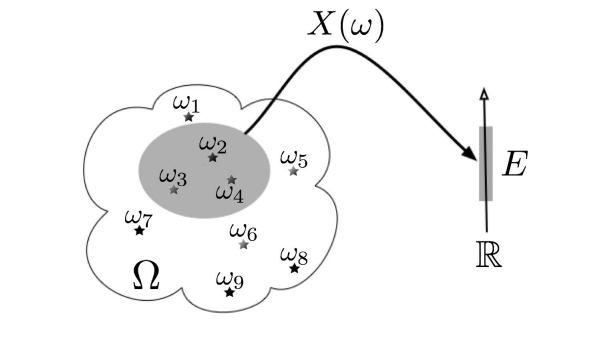
\includegraphics[width=0.3\linewidth]{images/random_variables.png}
    \caption{A visual idea of what is a random variable.}
    \label{fig:random_variables}
\end{figure}
\noindent Since this mapping describes the probability of the random variable $\displaystyle X$ falling within a subset of $\displaystyle \mathbb{R}$, it is possible to define the pre-image of a set $\displaystyle E \subseteq \mathbb{R}$ as the set $\displaystyle X^{-1}(E) = \{\omega \in \Omega : X(\omega) \in E\} \subseteq \Omega$. \newline
This definition allows to describe the probability distribution of a random variable $\displaystyle X$ as
\[\mathbb{P}(X \in E) = \mathbb{P}(\{\omega \in \Omega : X(\omega) \in E\}) = \mathbb{P}(X^{-1}(E))\]
\begin{figure}[H]
    \centering
    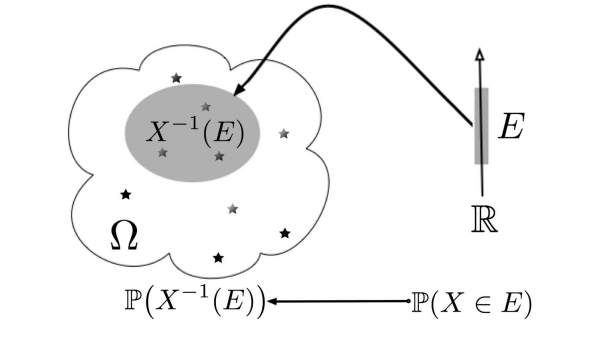
\includegraphics[width=0.3\linewidth]{images/random_variables_pullback.png}
    \caption{A visual idea of the pre-image of a random variable.}
    \label{fig:placeholder}
\end{figure}
\noindent When defining the probability distribution of a random variable $\displaystyle X$, it should be noticed that $\displaystyle \mathbb{P}(X \in E)$ represents an induced distribution supported on $\displaystyle \mathbb{R}$ that is constructed based on the assumed distribution $\displaystyle \mathbb{P}(X^{-1}(E))$ supported on $\displaystyle \Omega$.
\subsection{Discrete random variables}
A random variable is said to be ``discrete'' if its support is a countable set, which means that the random variable can take at most a finite, or at least countable, number of values. \newline
For this reason, a discrete random variable $\displaystyle X: \Omega \to S_X$ can be described using a probability mass function $\displaystyle p_X(x) = \mathbb{P}(X = x)$ that satisfies the following conditions:
\begin{itemize}
    \item $\displaystyle p_X(x) \ge 0 \text{ } \forall x \in \mathbb{R}$, with $\displaystyle p_X(x) > 0 \text{ } \forall x \in S_X$ specifically.
    \item $\displaystyle \sum_{x \in S_X} p_X(x) = 1$.
\end{itemize}
\begin{examplebox}[Repeated coin flips]
    Consider $\displaystyle 5$ independent flips of a fair coin: since each flip can be seen as a repetition of a binary experiment with sample space $\displaystyle \Omega = \{Heads, Tails\}$, it is possible to define the overall outcome space as the Cartesian product $\displaystyle \Omega^{\otimes 5}$. \newline
    Assuming symmetry and independence between coin flips, each outcome $\displaystyle \omega \in \Omega^{\otimes 5}$ is equally likely and has probability $\displaystyle \mathbb{P}(\omega) = \frac{1}{|\Omega^{\otimes 5}|} = \frac{1}{32}$. \newline
    Define now the random variable $\displaystyle X = \{\text{Number of tails in $5$ independent coin flips}\}$: on its support $\displaystyle S_X = \{0, 1, 2, 3, 4, 5\}$, the probability definition of $\displaystyle X$ can be defined as
    \[p_X(x) = \mathbb{P}(X = x) = \binom{5}{x}\bigg(\frac{1}{2}\bigg)^5 \text{, for $x \in S_X$.}\]
\end{examplebox}
\subsection{Continuous random variables}
A random variable is said to be ``continuous'' if its support is an uncountable set. \newline
Since, in this setting, $\displaystyle \mathbb{P}(X = x) \to 0 \text{ } \forall x \in \mathbb{R}$, a continuous random variable $\displaystyle X: \Omega \to S_X$ is described using a probability density function $\displaystyle f_X(x)$ that satisfies the following conditions:
\begin{itemize}
    \item $\displaystyle \mathbb{P}(a \leq X \leq b) = \mathbb{P}(X \in [a, b]) = \int_a^b f_X(x) \ dx$.
    \item $\displaystyle f_X(x) \ge 0 \text{ } \forall x \in \mathbb{R}$, with $\displaystyle f_X(x) > 0 \text{ } \forall x \in S_X$ specifically.
    \item $\displaystyle \int_{\mathbb{R}} f_X(x) = 1$.
\end{itemize}
In particular, all information about a continuous random variable $\displaystyle X$ can be retrieved from its cumulative distribution function $\displaystyle F_X: \mathbb{R} \to [0, 1]$, which can be defined as
\[F_X(x) = \mathbb{P}(X \leq x) = \mathbb{P}(X \in (-\infty, x]) \text{ } \forall x \in \mathbb{R}\]
More specifically, a function $\displaystyle F_X: \mathbb{R} \to [0, 1]$ acts as a cumulative distribution function on some probability measure $\displaystyle \mathbb{P}$ if and only if the following conditions are met:
\begin{itemize}
    \item $\displaystyle F_X(x)$ is non-decreasing, which means that $\displaystyle F_X(x_1) \leq F_X(x_2) \text{ } \forall x_1 < x_2$.
    \item $\displaystyle F_X(x)$ is normalized, meaning that
    \[\lim_{x \to -\infty} F_X(x) = 0 \quad\quad\quad \lim_{x \to +\infty} F_X(x) = 1\]
    \item $\displaystyle F_X(x)$ is right-continuous, which means that
    \[F_X(x) = F_X(x^+)= \lim_{t \to x^+} F_X(t)\]
\end{itemize}
Furthermore, the cumulative distribution function of a random variable $\displaystyle X$ always satisfies several properties:
\begin{itemize}
    \item $\displaystyle \mathbb{P}(x_1 < X \leq x_2) = \mathbb{P}(X \in (x_1, x_2]) = F(x_2) - F(x_1)$.
    \item $\displaystyle \mathbb{P}(X > x) = \mathbb{P}(X \in (x, +\infty)) = 1 - F_X(x)$.
    \item If $\displaystyle X$ is a continuous random variable with probability density function $\displaystyle f_X(x)$, then
    \[F_X(x) = \int_{-\infty}^x f_X(t) \ dt \text{ and } f_X(x) = F'(x) \text{ wherever $F_X$ is differentiable.}\]
    It should be noticed that this last property can also be formulated for discrete random variables. \newline
    In fact, if $\displaystyle X$ is a discrete random variable with probability mass function $\displaystyle p_X(x)$, then its cumulative function is given by
    \[F_X(x) =\sum_{x_i \leq x} p_X(x_i) = \mathbb{P}(X < x) + p_X(x) \text{, with $p_X(x) = F_X(x) - F_X(x^-)$.}\]
\end{itemize}
\begin{examplebox}[Playing darts]
    Suppose you throw a dart on a disc of radius $\displaystyle r$ at random. \newline
    Define the random variable $\displaystyle X = \{\text{Distance of the hitting point from the center}\}$ and note that its support $\displaystyle [0, r]$ is an uncountable set.
    \begin{align*}
        \mathbb{P}(X \leq x) &= 0 \text{ } \forall x < 0 \text{ as distances are not negative.} \\
        \mathbb{P}(X \leq x) &= 1 \text{ } \forall x > r \text{ as the dart did hit the disc.} \\
        \mathbb{P}(X \leq x) &= \frac{\pi x^2}{\pi r^2} = \frac{x^2}{r^2} \text{ } \forall x \in [0, r]
    \end{align*}
    Therefore, it is possible to define the cumulative distribution function of $\displaystyle X$ as
    \[F_X(x) = \begin{cases}
        0 &\quad\text{if $x < 0$} \\
        \frac{x^2}{r^2} &\quad\text{if $x \in [0, r]$} \\
        1 &\quad\text{if $x > r$} \\
    \end{cases}\]
    This implies that the probability density function will be
    \[f_X(x) = \begin{cases}
        \frac{2x}{r^2} &\quad\text{if $x \in [0, r]$} \\
        0 &\quad\text{otherwise} \\
    \end{cases} \text{, or } f_X(x) = \frac{2x}{r^2}\mathbb{I}_{[0, r]}(x) \text{, with } \mathbb{I}_{[0, r]}(x) = \begin{cases}
        1 &\quad\text{if $x \in [0, r]$} \\
        0 &\quad\text{otherwise}
    \end{cases}\]
\end{examplebox}
\section{The quantile function of a random variable}
Let $\displaystyle X: \Omega \to S_X$ be a continuous random variable with cumulative distribution function $\displaystyle F_X(x)$: for a given level $\displaystyle p \in [0, 1]$, the quantile function is defined as
\[q_p = \mathbb{Q}(p) = \inf\{x \in S_X: F_X(x) = p\}\]
In particular, if $\displaystyle F_X(x)$ is strictly increasing in $\displaystyle \mathbb{R}$, then it is also invertible and it is possible to set
\[q_p = \mathbb{Q}(p) = F_X^{-1}(p) \text{ and } p = F_X(q_p) = \int_{-\infty}^{q_p} f_X(t) \ dt \text{.}\]
\begin{examplebox}[The median of a Pareto distribution]
    A continuous random variable $\displaystyle X$ is said to follow a Pareto distribution with parameter $\displaystyle \alpha > 0$ if its cumulative distribution function is defined as
    \[F_X(x) = \begin{cases}
        0 &\quad\text{if $x < 1$} \\
        1 - \frac{1}{x^\alpha} &\quad\text{if $x \ge 1$} \\
    \end{cases}\]
    Assuming $\displaystyle \alpha = 0.5$, suppose you want to find the median of the distribution: since $\displaystyle F_X(x)$ is strictly increasing in $\displaystyle [1, +\infty)$, it is possible to find
    \[F(q_p) = 1 - \frac{1}{\sqrt{q_p}} = \frac{\sqrt{q_p} - 1}{\sqrt{q_p}} = 0.5 \Rightarrow 0.5\sqrt{q_p} = \sqrt{q_p} - 1 \Rightarrow 0.5\sqrt{q_p} = 1 \Rightarrow q_p = 4\]
\end{examplebox}
\noindent However, since discrete random variables tend to have weakly monotonic cumulative distribution functions, a more general definition of quantile function is typically used. \newline
In fact, given any random variable $\displaystyle X: \Omega \to S_X$ with cumulative distribution function $\displaystyle F_X(x)$, the quantile function for a given level $\displaystyle p \in [0, 1]$ is formulated as
\[q_p = \mathbb{Q}(p) = \inf\{x \in S_X : F_X(x) \ge p\}\]
\begin{examplebox}[The median of a discrete distribution]
    Let $\displaystyle X$ be a discrete random variable whose probability distribution is given by
    \[p_X(x) = \begin{cases}
        \frac{2}{5} &\quad\text{if $x = -1$} \\
        \frac{1}{5} &\quad\text{if $x = 0$} \\
        \frac{2}{5} &\quad\text{if $x = 1$} \\
    \end{cases} \quad\quad\quad F_X(x) = \begin{cases}
        0 &\quad\text{if $x < -1$} \\
        \frac{2}{5} &\quad\text{if $x \in [-1, 0)$} \\
        \frac{3}{5} &\quad\text{if $x \in [0, 1)$} \\
        1 &\quad\text{if $x \ge 1$} \\
    \end{cases}\]
    Suppose you want to find the median of the distribution: since $\displaystyle F_X(x)$ is not strictly increasing, it is necessary to use the general definition of quantile function to find
    \[q_p = \inf\{x \in S_X : F_X(x) \ge 0.5\} = 0\]
\end{examplebox}
\section{Common univariate distributions}
Sometimes, the behaviour of a random variable can be described by some known theoretical probability distribution.
\subsection{The Bernoulli distribution}
A discrete random variable $\displaystyle X$ is said to follow a Bernoulli distribution with parameter $\displaystyle p \in [0, 1]$, which is written as $\displaystyle X \sim Ber(p)$, if its probability mass function is defined as
\[p_X(x) = p^x(1 - p)^{1 - x} \text{, for $x \in \{0, 1\}$.}\]
\begin{figure}[H]
    \centering
    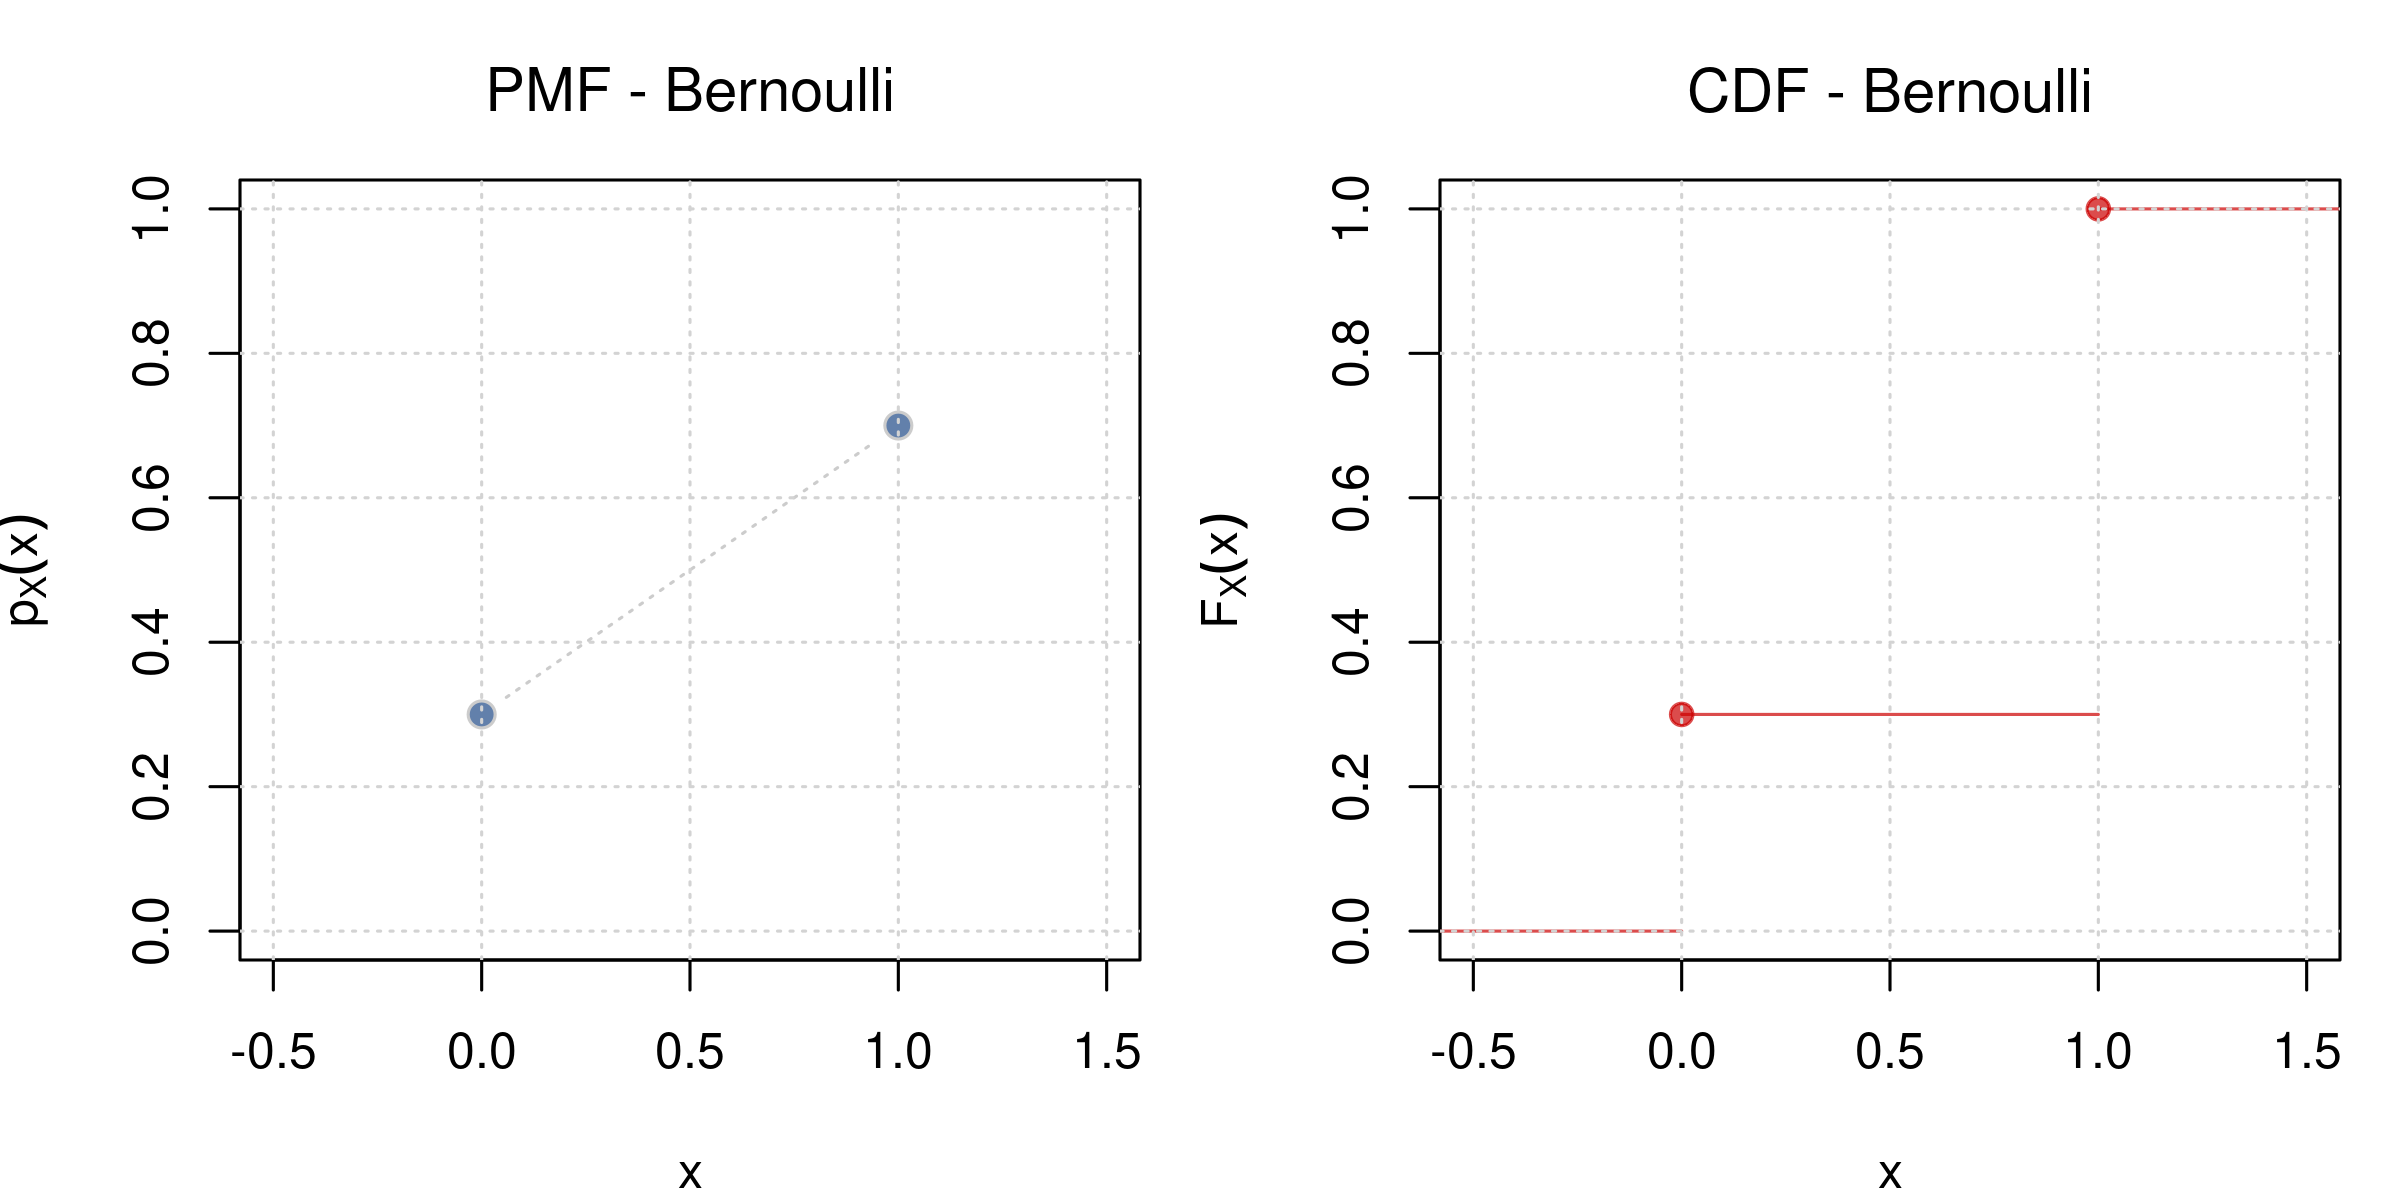
\includegraphics[width=0.5\linewidth]{images/bernoulli.png}
    \caption{PMF and CDF for a random variable $\displaystyle X \sim Ber(0.7)$.}
    \label{fig:bernoulli}
\end{figure}
\noindent For this reason, Bernoulli random variables come in handy to model binary experiments whose only possible outcomes are success, which is denoted by $\displaystyle X = 1$, and failure, which is denoted by $\displaystyle X = 0$.
\begin{examplebox}[Logistic regression]
    Logistic regression is a classification model that aims to predict a binary label $\displaystyle y$ based on a feature vector $\displaystyle \mathbf{x}$. \newline
    For this reason, it is possible to model a conditional probability $\displaystyle \mathbb{P}(y|\mathbf{x}) \sim Ber(p(\mathbf{x}))$ whose success probability is computed using the logistic function
    \[\ln\bigg(\frac{p(\mathbf{x})}{1 - p(\mathbf{x})}\bigg) = \alpha + \mathbf{\beta}^T\mathbf{x} \Rightarrow p(\mathbf{x}) = \frac{e^{\alpha + \mathbf{\beta}^T\mathbf{x}}}{1 + e^{\alpha + \mathbf{\beta}^T\mathbf{x}}}\]
\end{examplebox}
\noindent Moreover, if $\displaystyle X$ is a random variable with probability density function $\displaystyle f_X(x)$, or probability mass function $\displaystyle p_X(x)$, then, for some event $\displaystyle A$, it holds that $\displaystyle Y = r(X) = \mathbb{I}_A(X) \sim Ber(p)$, with
\[p = \int_A f_X(x) \ dx\]
\subsection{The binomial distribution}
A discrete random variable $\displaystyle X$ is said to follow a binomial distribution with parameters $\displaystyle n \in \mathbb{N}_0$ and $\displaystyle p \in [0, 1]$, which is written as $\displaystyle X \sim Bin(n, p)$, if its probability mass function is defined as
\[p_X(x) = \binom{n}{x}p^x(1 - p)^{n - x} \text{, for $x \in \{0, \dots, n\}$.}\]
\begin{figure}[H]
    \centering
    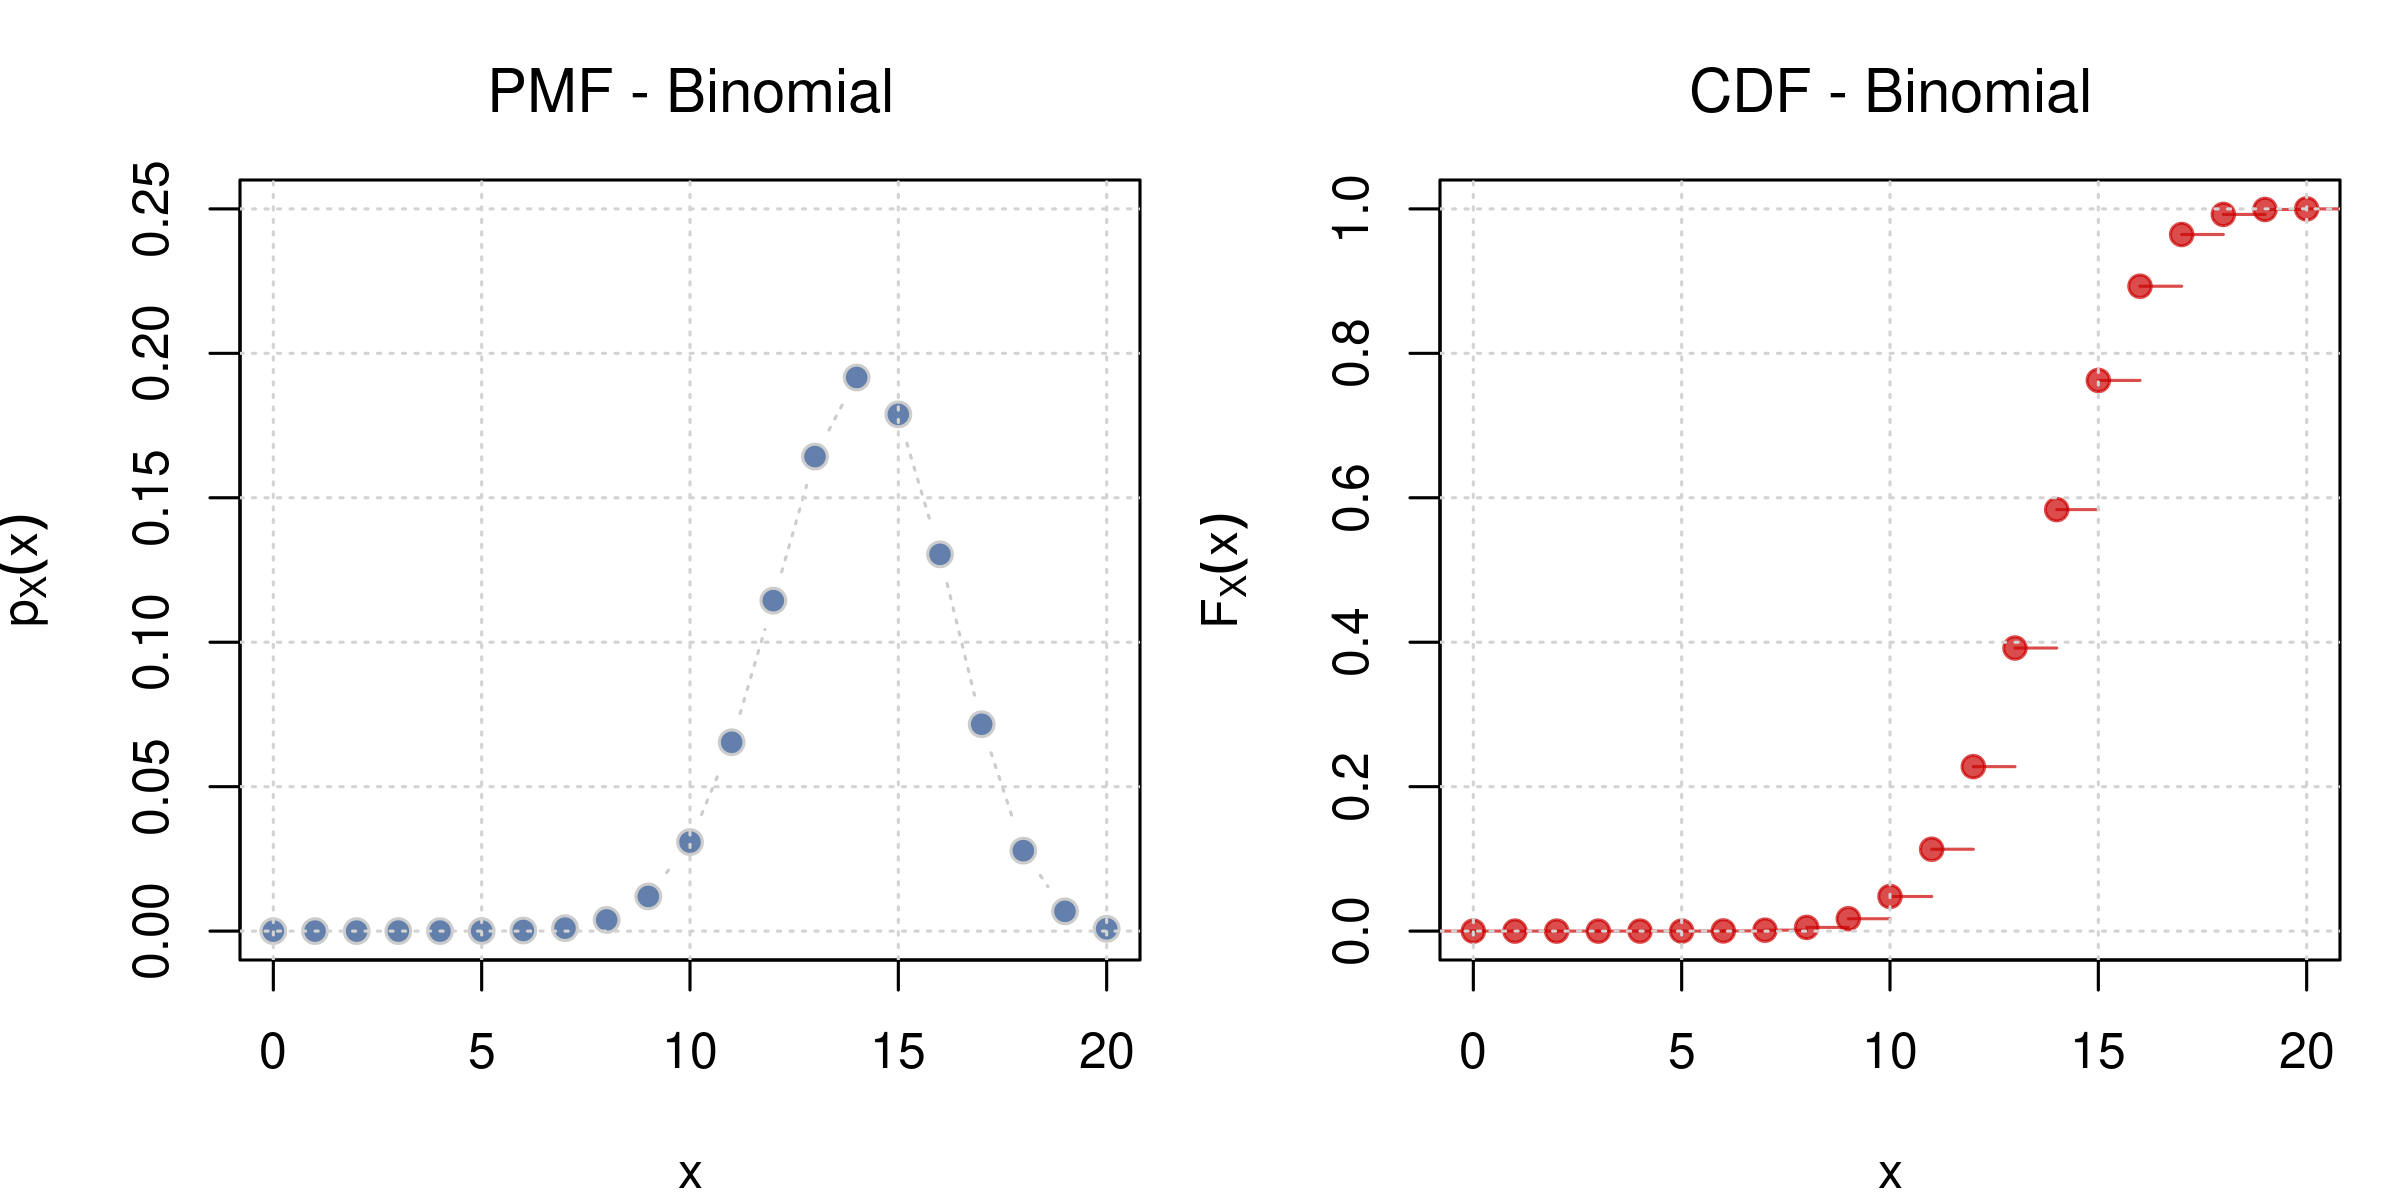
\includegraphics[width=0.5\linewidth]{images/binomial.png}
    \caption{PMF and CDF for a random variable $\displaystyle X \sim Bin(20, 0.7)$.}
    \label{fig:binomial}
\end{figure}
\noindent Since binomial random variables are often used to model experiments counting the number of successful attempts out of $\displaystyle n$ independent and identically distributed Bernoulli trials with success probability $\displaystyle p$, it is also possible to define a random variable $\displaystyle X \sim Bin(n, p)$ as
\[X = \sum_{i = 1}^n X_i \text{, with $X_i \sim Ber(p) \text{ } \forall i \in \{1, \dots, n\}$.}\]
\begin{examplebox}[Guessing card symbols]
    A man who claims to be a psychic is asked to guess the symbols drawn on $\displaystyle 25$ cards. \newline
    Since the man guesses at random with success probability $\displaystyle p = 0.7$ at each round, define the random variable $\displaystyle X_i = \{\text{The $i^{th}$ guess is correct}\}$ and note that $\displaystyle X_i \sim Ber(p) \text{ } \forall i \in \{1, \dots, 25\}$. \newline
    For this reason, the random variable $\displaystyle X = \{\text{Total correct guesses}\}$ can be formulated as
    \[X = \sum_{i = 1}^{25} X_i \Rightarrow X \sim Bin(25, 0.7) \Rightarrow p_X(x) = \binom{25}{x}(0.7)^x(0.3)^{25 - x} \text{, for $x \in \{0, \dots, 25\}$.}\]
    This means that the probability that the man correctly guesses each symbol will be
    \[p_X(25) = \binom{25}{25}(0.7)^{25}(0.3)^{25 - 25} = (0.7)^{25} \approx 1.34 \cdot 10^{-4}\]
\end{examplebox}
\subsection{The uniform distribution}
A continuous random variable $\displaystyle X$ is said to follow a uniform distribution with parameters $\displaystyle a < b \in \mathbb{R}$, which is written as $\displaystyle X \sim Unif(a, b)$, if its probability density function and cumulative distribution function are defined as
\[f_X(x) = \frac{1}{b - a}\mathbb{I}_{[a, b]}(x) \quad\quad\quad F_X(x) = \begin{cases}
    0 &\quad\text{if $x < a$} \\
    \frac{x - a}{b - a} &\quad\text{if $x \in [a, b]$} \\
    1 &\quad\text{if $x > b$} \\
\end{cases}\]
\begin{figure}[H]
    \centering
    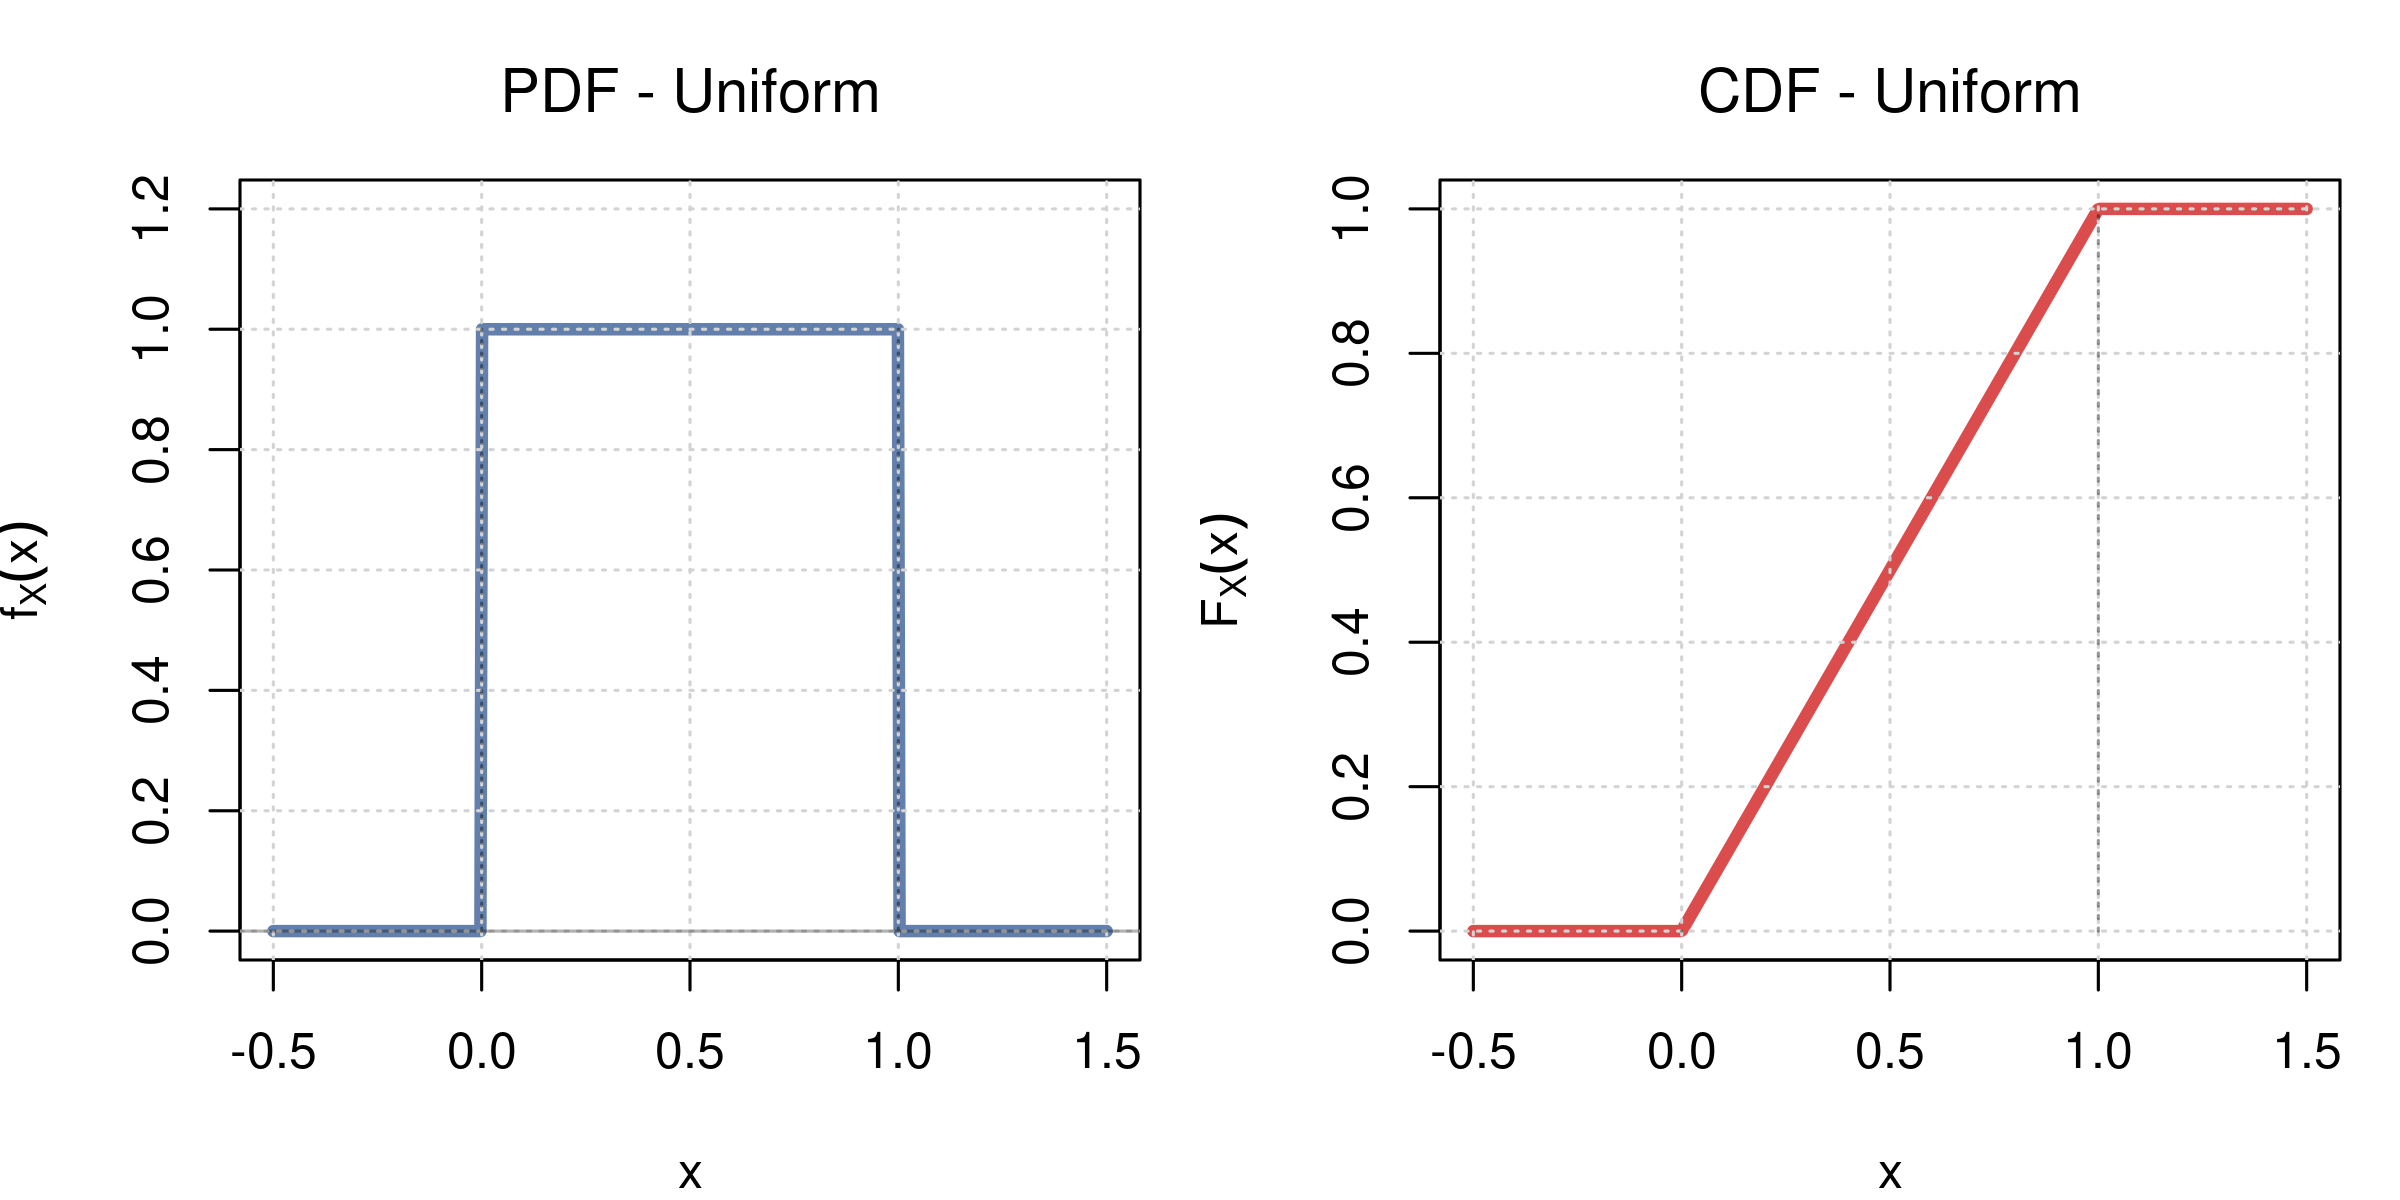
\includegraphics[width=0.5\linewidth]{images/uniform.png}
    \caption{PDF and CDF for a random variable $\displaystyle X \sim Unif(0, 1)$.}
    \label{fig:uniform}
\end{figure}
\noindent An important application of the uniform distribution consists of generating random variables for simulation modelling. \newline
Given a random variable $\displaystyle U \sim Unif(0, 1)$, let $\displaystyle F$ be a cumulative distribution function with quantile function $\displaystyle \mathbb{Q}$: the ``quantile transform'' $\displaystyle Y = \mathbb{Q}(U)$ will be a random variable with cumulative distribution function $\displaystyle F_Y(y) = F$.
\begin{proofbox}
    Assuming $\displaystyle F$ is continuous and strictly increasing, it is possible to exploit the fact that $\displaystyle \mathbb{Q} = F^{-1}$ to let
    \[F_Y(y) = \mathbb{P}(Y \leq y) = \mathbb{P}(F^{-1}(U) \leq y) = \mathbb{P}(U \leq F(y)) = F(y) \text{, being $U \sim Unif(0, 1)$.}\]
    It should be noticed that this result is also valid whenever $\displaystyle F$ is only weakly monotonic, although the proof is more cumbersome.
\end{proofbox}

\chapter{Random vectors}
\section{Defining random vectors}
Given a probability space $\displaystyle (\Omega, \mathbb{P})$, a random vector, also known as a $\displaystyle p$-variate random variable, is a (measurable) mapping $\displaystyle \mathbf{X}: \Omega \to \mathbb{R}^p$ that maps every outcome $\displaystyle \omega \in \Omega$ onto a vector $\displaystyle \mathbf{X}(\omega) \in \mathbb{R}^p$. \newline
Generally speaking, the behaviour of a random vector, whose components can be studied individually through univariate analysis or jointly by analysing dependencies between single variables, is defined by its joint distribution, which is normally represented as a contingency table or tensor. \newline
Furthermore, the joint distribution of a random vector can be used to derive the marginal distributions, which describe the behaviour of a single variable, and to model conditional distributions, which describe the behaviour of a variable conditioned to a given event. \newline
Overall, random vectors can be seen as a generalization of random variables and, while they are mainly used to study bivariate distributions, their behaviour and properties can be extended to analyse $\displaystyle p > 2$ variables as well.
\section{Fully discrete random vectors}
A random vector is said to be ``fully discrete'' if all its components are discrete random variables. \newline
For a bivariate distribution, the behaviour of a random vector $\displaystyle \mathbf{Z}$ is described using a joint probability mass function
\[p_{\mathbf{Z}}(\mathbf{z}) = p_{X, Y}(x, y) = \mathbb{P}(\{X = x\} \cap \{Y = y\}) \text{ } \forall (x, y) \in S_X \times S_Y\]
Starting from the joint distribution, it is possible to retreive the marginal distribution of a single variable by computing
\begin{align*}
    p_X(x) &= \mathbb{P}\Bigg(\{X = x\} \cap \Bigg(\bigcup_{y \in S_Y} \{Y = y\}\Bigg)\Bigg) = \bigcup_{y \in S_Y} \mathbb{P}(\{X = x\} \cap \{Y = y\}) = \sum_{y \in S_Y} p_{X, Y}(x, y) \\
    p_Y(y) &= \mathbb{P}\Bigg(\Bigg(\bigcup_{x \in S_X} \{X = x\}\Bigg) \cap \{Y = y\}\Bigg) = \bigcup_{x \in S_X} \mathbb{P}(\{X = x\} \cap \{Y = y\}) = \sum_{x \in S_X} p_{X, Y}(x, y)
\end{align*}
Furthermore, assuming a certain event has occurred, it is possible to model the conditional distribution of each variable as
\begin{align*}
    p_{X|Y}(x|y) &= \mathbb{P}(X = x|Y = y) = \frac{\mathbb{P}(\{X = x\} \cap \{Y = y\})}{\mathbb{P}(Y = y)} = \frac{p_{X, Y}(x, y)}{p_Y(y)} \text{ } \forall x \in S_X \\
    p_{Y|X}(y|x) &= \mathbb{P}(Y = y|X = x) = \frac{\mathbb{P}(\{X = x\} \cap \{Y = y\})}{\mathbb{P}(X = x)} = \frac{p_{X, Y}(x, y)}{p_X(x)} \text{ } \forall y \in S_Y
\end{align*}
\begin{examplebox}[The relationship between exam results and class attendance]
    Consider the random variables $\displaystyle X = \{\text{I pass the exam}\}$, whose support set is $\displaystyle S_X = \{0, 1\}$, and $\displaystyle Y = \{\text{I attend classes}\}$, whose support set is $\displaystyle S_Y = \{N, S, A\}$: on the set $\displaystyle S_X \times S_Y$, their joint distribution is defined as
    
    {\centering
    \vspace{0.5em}
    \begin{tabular}{|l|c c c|r|}
        \hline
        & \multicolumn{3}{c|}{$Y$} & \\
        \hline
        $X$ & $N$ & $S$ & $A$ & \textbf{Total} \\
        \hline
        $0$ & $0.6$ & $0.05$ & $0.05$ & $0.7$ \\
        $1$ & $0.2$ & $0.01$ & $0.09$ & $0.3$ \\
        \hline
        \textbf{Total} & $0.8$ & $0.06$ & $0.14$ & $1.0$ \\
        \hline
    \end{tabular}
    \vspace{0.5em}\par}
    
    \noindent Looking at the contingency table, it is possible to recover the joint distributions
    \begin{align*}
        p_X(x) &= \sum_{y \in S_Y} p_{X, Y}(x, y) = \begin{cases}
            0.7 &\quad\text{if $x = 0$} \\
            0.3 &\quad\text{if $x = 1$} \\
        \end{cases} \\
        p_Y(y) &= \sum_{x \in S_X} p_{X, Y}(x, y) = \begin{cases}
            0.8 &\quad\text{if $y = N$} \\
            0.06 &\quad\text{if $y = S$} \\
            0.14 &\quad\text{if $y = A$} \\
        \end{cases}
    \end{align*}
    Furthermore, it is possible to define the conditional distribution of $\displaystyle X$ given the event $\displaystyle \{Y = y\}$, with $\displaystyle y \in S_Y$, as
    \begin{align*}
        p_{X|Y}(x|Y = N) &= \mathbb{P}(X = x|Y = N) = \begin{cases}
            0.75 &\quad\text{if $x = 0$} \\
            0.25 &\quad\text{if $x = 1$}
        \end{cases} \\
        p_{X|Y}(x|Y = S) &= \mathbb{P}(X = x|Y = S) = \begin{cases}
            0.83 &\quad\text{if $x = 0$} \\
            0.17 &\quad\text{if $x = 1$}
        \end{cases} \\
        p_{X|Y}(x|Y = A) &= \mathbb{P}(X = x|Y = A) = \begin{cases}
            0.36 &\quad\text{if $x = 0$} \\
            0.64 &\quad\text{if $x = 1$}
        \end{cases}
    \end{align*}
\end{examplebox}
\subsection{Defining independence for discrete random variables}
When working with (bivariate) random vectors, two random variables $\displaystyle X$ and $\displaystyle Y$ are independent if and only if their joint probability mass function factorises to the product of their marginal probability mass functions, meaning that
\[p_{X, Y}(x, y) = p_X(x)p_Y(y) \text{ } \forall (x, y) \in S_X \times S_Y\]
Alternatively, it is possible to state that two random variables $\displaystyle X$ and $\displaystyle Y$ are independent if and only if their conditional distributions correspond to the marginal distributions, meaning that
\[p_{X|Y}(x|y) = p_X(x) \quad\quad p_{Y|X}(y|x) = p_Y(y) \]
\begin{examplebox}[Exam results and class attendance as independent random variables]
    Consider the random variables $\displaystyle X = \{\text{I pass the exam}\}$, whose support set is $\displaystyle S_X = \{0, 1\}$, and $\displaystyle Y = \{\text{I attend classes}\}$, whose support set is $\displaystyle S_Y = \{N, S, A\}$: assuming the two random variables are independent, their joint distribution becomes
    
    {\centering
    \vspace{0.5em}
    \begin{tabular}{|l|c c c|r|}
        \hline
        & \multicolumn{3}{c|}{$Y$} & \\
        \hline
        $X$ & $N$ & $S$ & $A$ & \textbf{Total} \\
        \hline
        $0$ & $0.56$ & $0.042$ & $0.098$ & $0.7$ \\
        $1$ & $0.24$ & $0.018$ & $0.042$ & $0.3$ \\
        \hline
        \textbf{Total} & $0.8$ & $0.06$ & $0.14$ & $1.0$ \\
        \hline
    \end{tabular}
    \vspace{0.5em}\par}
    
    \noindent Generally speaking, it is possible to check how much two random variables are far from independence by evaluating the distance between their joint distribution $\displaystyle p_{X, Y}$ and the factorised distribution $\displaystyle \tilde{p}$.
\end{examplebox}
\section{Fully continuous random vectors}
A random vector is said to be ``fully continuous'' if all its components are continuous random variables.
\section{The cumulative distribution function of a joint distribution}
Generally speaking, the joint cumulative distribution function of any bivariate random vector is defined as
\[F_{X, Y}(x, y) = \mathbb{P}(\{X \leq x\} \cap \{Y \leq y\}) \text{ } \forall (x, y) \in S_X \times S_Y\]
In this case, it is possible to retrieve the marginal cumulative distribution functions by computing
\begin{align*}
    F_X(x) &= \lim_{y \to +\infty} F_{X, Y}(x, y) \text{ } \forall x \in S_X \\
    F_Y(y) &= \lim_{x \to +\infty} F_{X, Y}(x, y) \text{ } \forall y \in S_Y
\end{align*}
Furthermore, whenever two random variables $\displaystyle X$ and $\displaystyle Y$ are independent, it is the case that
\[F_{X, Y}(x, y) = F_X(x)F_Y(y) \text{ } \forall (x, y) \in \mathbb{R}^2\]
\subsection{Building independent and identically distributed random samples}
A random sample $\displaystyle \mathcal{D}_n = \{X_1, \dots, X_n\}$ is said to be ``independent and identically distributed'' if all the sampled random variables are independent and come from the same population model $\displaystyle F_X$, allowing to define their joint distribution as
\[\mathbb{P}(\mathcal{D}_n) = F(x_1, \dots, x_n) = \mathbb{P}(X_1 \leq x_1, \dots, X_n \leq x_n) = \prod_{i = 1}^n \mathbb{P}(X_i \leq x_i) = \prod_{i = 1}^n F(x_i)\]
\begin{examplebox}[Maximum likelihood estimation]
    Consider a machine learning model that aims to learn an unknown population model $\displaystyle F_X$ from a random sample $\displaystyle \mathcal{D}_n$: using the likelihood function leads the model to learn the empirical cumulative distribution function associated to a distribution that places the same mass to each data point, meaning that
    \[\hat{F} = \arg\max_{F_X \text{ CDF}} L(F_X) = \arg\max_{F_X \text{ CDF}} \prod_{i = 1}^n F_X(x_i)\]
\end{examplebox}
\noindent This concept can be generalized to create random samples of random vectors as well.

\chapter{Stochastic simulations}
\section{Defining simulations}
A stochastic simulation allows to study complex probabilistic models by generating values for a random variable that will be used into the model, providing an approximation of a random system. \newline
Simulations come in handy to investigate the typical behaviour of a system and its fluctuations, although more advanced techniques can be integrated to study exceptional cases as well.
\begin{examplebox}[A physical simulation]
    Suppose you want to create a simulation of a balanced coin flip based on the result seen by tossing a fair die: a possible strategy could consist of having the coin show heads when the die shows an odd result, or tails when the die shows an even result. \newline
    Alternatively, it is possible to simulate the result shown by the die by (repeatedly) tossing the coin and associating each sequence of outcomes to a certain value.
\end{examplebox}
\section{Pseudorandom number generators}
A pseudorandom number generator is a deterministic algorithm that, starting from an initial ``seed'' $\displaystyle u_0$, produces a sequence of numbers that resembles a random sequence. \newline
For this reason, a pseudorandom number generator can be modelled as a function $\displaystyle \mathbf{f}: (0, 1) \to (0, 1)$ such that, for any seed $\displaystyle u_0$, the resulting sequence
\[\{u_0, \mathbf{f}(u_0), \dots, \mathbf{f}^n(u_0)\} \text{ behaves like a $Unif(0, 1)$ independent and identically distributed sequence.}\]
A common method for pseudorandom number generation is the linear congruential generator, which, on the set $\displaystyle \{1, \dots, M\}$, is defined as
\[\mathbf{f}(x) = (\alpha + \beta x) \bmod M\]
\begin{lstlisting}[
  language=R,
  captionpos=b,
  caption={R implementation of a linear congruential generator.},
  label={lst:lcg}
]
    lcg <- function(u0, n=1000, a=69069069, b=12345, M=2^32){
      x_out <- rep(NA, n)
      x_out[1] <- u0
      for (i in 2:n) {
        x_out[i] <- (a + (b * x_out[i - 1])) %% M
      }
      return(x_out / (M + 1))
    }
\end{lstlisting}
\noindent In fact, this function acts as a generator on $ \displaystyle (0, 1)$ when scaled by $\displaystyle (M + 1)$.
\begin{examplebox}[A simple linear congruential generator]
    Consider the linear congruential generator
    \[\mathbf{f}(x) = (69069069x + 12345) \bmod 2^{32}\]
    For a given $\displaystyle u_0$, the function generates the sequence
    \[518974515, 2498053016, 1113825472, 1109377984, \dots \text{, which can be scaled to}\]
    \[0.1208332, 0.5816233, 0.2593327, 0.2592972, \dots\]
\end{examplebox}
\noindent The quality of a linear congruential generator can be evaluated using the Chebyshev distance between the target probability density function $\displaystyle f_u$ and the generated probability density function $\displaystyle \hat{f}$, which is defined as
\[D(f_u, \hat{f}) = \max_{u \in \mathbb{R}} |f_u(u) - \hat{f}(u)|\]
Ideally, a well-performing linear congruent generator should achieve consistent convergence, which means that, for any data sequence, the maximum loss approaches $\displaystyle 0$ as the sequence grows infinitely large, meaning that
\[\max_{\text{all data}} D(f_u, \hat{f}) \xrightarrow{n \to +\infty} 0\]
Most of the time, however, it is sufficient to have the average error to vanish for a linear congruential generator to be good.
\subsection{The period of a linear congruential generator}
For certain choices of $\displaystyle \alpha$ and $\displaystyle \beta$, a linear congruential generator has a period equal to $\displaystyle M$ and, when scaled by $\displaystyle (M + 1)$, it can act as a generator on $\displaystyle (0, 1)$. \newline
More specifically, a linear congruential generator has a period equal to $\displaystyle M$ for any starting seed $\displaystyle u_0$ if and only if:
\begin{itemize}
    \item $\displaystyle M$ and $\displaystyle \alpha$ are co-prime, which means that $\displaystyle \text{GCD}(M, \alpha) = 1$.
    \item $\displaystyle (\beta - 1)$ is divisible by all prime factors of $\displaystyle M$.
    \item $\displaystyle (\beta - 1)$ is a multiple of $\displaystyle 4$ if $\displaystyle M$ is a multiple of $\displaystyle 4$.
\end{itemize}
\subsection{The distribution of a linear congruential generator}
Generally speaking, it is possible to assess whether the generated random variable produces a sequence resembling a $\displaystyle Unif(0, 1)$ random sample through dedicated statistical tests.
\subsection{Simulating independence in a linear congruential generator}
Since each generated sample $\displaystyle u_n$ is a deterministic function of the previous value $\displaystyle u_{n - 1}$, linear congruential generators tend to create dependent sequences. \newline
To simulate independent samples, a linear congruential generator must be $\displaystyle k$-dimensionally equidistributed, with $\displaystyle k$ being chosen as a large value, which means that every subsequence of length $\displaystyle k$ occurs with equal frequency.
\section{Transformations of random variables}
It is possible to simulate (continuous) ransom variables through specific transformations.
\subsection{Using quantile transforms to generate populations}
The quantile transform can be used to create random variables starting from a $\displaystyle Unif(0, 1)$ generator.
\begin{examplebox}[Generating a continuous random variable]
    Let $\displaystyle X$ be a continuous random variable for which
    \[f_X(x) = 3x^2\mathbb{I}_{[0, 1]}(x) \text{ and } F_X(x) = \begin{cases}
        0 &\quad\text{if $x < 0$} \\
        x^3 &\quad\text{if $x \in [0, 1)$} \\
        1 &\quad\text{if $x \ge 1$} \\
    \end{cases}\]
    Since $\displaystyle F_X$ is an invertible function, it is possible to define the quantile function $\displaystyle \mathbb{Q}_X(p) = \sqrt[3]{p}$, with $\displaystyle p \in (0, 1)$. \newline
    Therefore, if $\displaystyle U \sim Unif(0, 1)$, the random variable $\displaystyle \sqrt[3]{U}$ follows the same distribution as $\displaystyle X$.
    \begin{figure}[H]
        \centering
        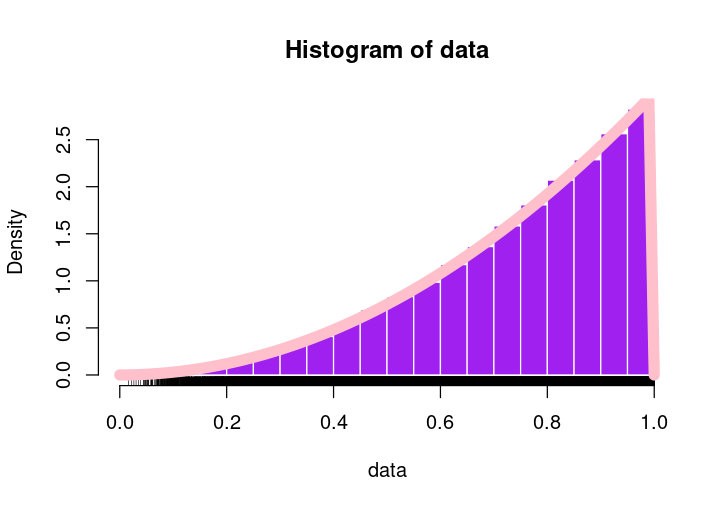
\includegraphics[width=0.35\linewidth]{images/population_generation_continuous.png}
        \caption{The distribution of $\displaystyle \sqrt[3]{U}$, with $\displaystyle U \sim Unif(0, 1)$.}
        \label{fig:population_continuous}
    \end{figure}
\end{examplebox}
\noindent While easy to implement, this algorithm becomes more cumbersome when generating discrete random variables.
\subsection{General transformation of random variables}
Starting from a continuous random variable $\displaystyle X$ that, on a support set $\displaystyle S_X$, has probability density function $\displaystyle f_X(x)$ and cumulative distribution $\displaystyle F_X(x)$, it is possible to study the random variable $\displaystyle Y = r(X)$ by defining the set $\displaystyle A_y = \{x \in S_X : r(x) \leq y\}$ and using it to compute
\begin{align*}
    F_Y(y) &= \mathbb{P}(Y \leq y) = \mathbb{P}(r(X) \leq y) = \mathbb{P}(\{x \in S_X : r(x) \leq y\}) = \int_{A_y} f_X(x) \ dx \\
    f_Y(y) &= F_Y'(y)\mathbb{I}_{S_Y}(y) \\
    S_Y &= \{r(x) : x \in S_X\}
\end{align*}
\begin{examplebox}[Transforming a uniformly distributed random variable]
    Given a random variable $\displaystyle X \sim Unif(-1, 1)$, define the random variable $\displaystyle Y = X^2$, whose cumulative distribution function is defined as
    \[F_Y(y) = \mathbb{P}(Y \leq y) = \mathbb{P}(X^2 \leq y) = \mathbb{P}(-\sqrt{y} \leq X \leq \sqrt{y}) = \int_{-\sqrt{y}}^{\sqrt{y}} \frac{1}{2} \ dx = \frac{x}{2}\Bigg|_{-\sqrt{y}}^{\sqrt{y}} = \sqrt{y}\]
    This means that, on the support $\displaystyle S_Y = \{x^2 : x \in S_X\} = [0, 1]$, the probability density function of $\displaystyle Y$ will be given by
    \[f_Y(y) = F_y'(y) = \frac{1}{2\sqrt{y}}\mathbb{I}_{(0, 1]}(y)\]
\end{examplebox}
\noindent However, if the function $\displaystyle r(x)$ is known to be invertible in $\displaystyle S_X$, with $\displaystyle s(y) = r^{-1}(x)$, it is possible to directly compute
\begin{align*}
    F_Y(y) &= \mathbb{P}(r(X) \leq y) = \mathbb{P}(X \leq s(y)) = F_X(s(y)) \\
    f_Y(y) &= F_Y'(y) = f_X(s(y)) \cdot s'(y)
\end{align*}

\end{document}